\subsubsection{Overview}

The B-Tree can be regarded as a function $\mathcal{F}$ that maps the key $x$ into its corresponding page index $y$. It is known to us that the pages are allocated in a way that the every $S$ entries are allocated in a page where $S$ is a pre-defined parameter. For example, if we set $S$ to be 10 items per page, then the first page will contain the first 10 keys and their corresponding values. Similarly, the second 10 keys and their corresponding values will be allocated to the second page.

If we know the CDF of $X$ as $F(X\leq x)$ and the total number of entries $N$, then the position of $x$ can be estimated as $p=F(x)*N$ and the page index where it should be allocated to is given by

$$y=\floor{\frac{p}{S}}=\floor{\frac{F(x)*N}{S}}$$  

\begin{mscexample}
For example, if the keys are uniformly distributed from $0$ to $1000$, i.e. the CDF of $X$ is defined as $F(X\leq x)=\frac{x}{1000}$ and we set $S=10, N=1001$. Then for any key $x$, we immediately know it will be allocated into $y=\floor{\frac{1000}{10}*\frac{x}{1000}}=\floor{\frac{x}{10}}$. Assume that we have a key $698$, then we can calculate $y=\floor{\frac{698}{10}}=69$. By doing so, the page index is calculated in constant time and space.

In this example, we see that the distribution of $X$ is essential and our goal of learned index in one-dimensional data is to learn such distribution. To do so, we apply two different techniques as the baseline, the polynomial regression and fully connected neural network.
\end{mscexample}

To train such a learned index, we first manually generate the $X$ with respect to a certain distribution. We then save the generated $X$ into a dense array with the length $N$. Then we use the proportional index, i.e. the index of each $x$ divided by $N$ as the expected output $y$.
 
\subsubsection{Fully Connected Neural Network}

After generating the training dataset $X$ and its corresponding $Y$, we build a fully connected neural network as the baseline learned index. The architecture of the fully connected neural network is illustrated in Figure \ref{fig:baseline_fcn}.

\tikzset{%
  every neuron/.style={
    circle,
    draw,
    minimum size=1cm
  },
  neuron missing/.style={
    draw=none, 
    scale=4,
    text height=0.333cm,
    execute at begin node=\color{black}$\vdots$
  },
}
\begin{figure}
\center
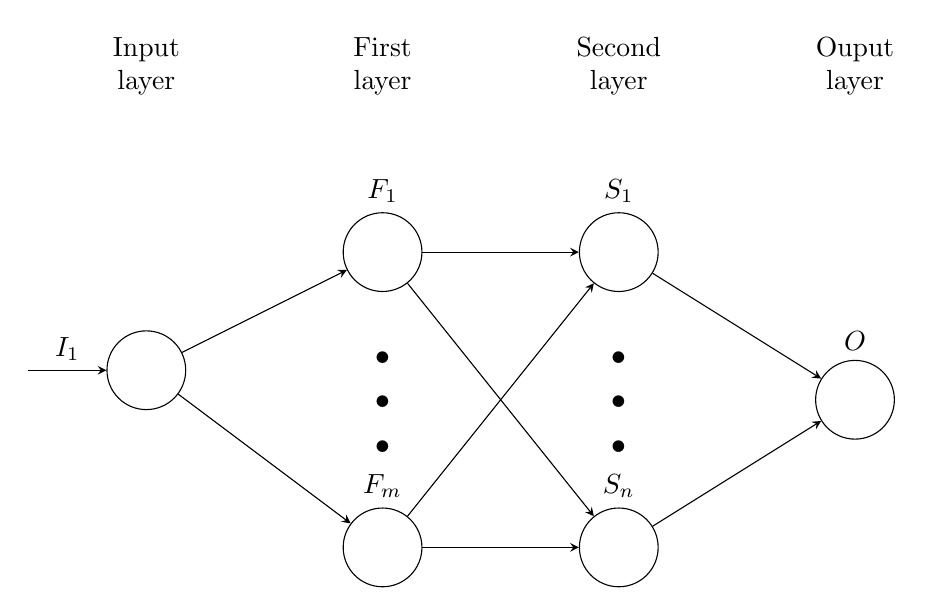
\begin{tikzpicture}[x=1.5cm, y=1.5cm, >=stealth]
\foreach \m/\l [count=\y] in {1}
  \node [every neuron/.try, neuron \m/.try] (input-\m) at (0,2.5-\y*2.75) {};

\foreach \m [count=\y] in {1,missing,2}
  \node [every neuron/.try, neuron \m/.try ] (first-\m) at (2,2-\y*1.25) {};

\foreach \m [count=\y] in {1,missing,2}
  \node [every neuron/.try, neuron \m/.try ] (second-\m) at (4,2-\y*1.25) {};

\foreach \m [count=\y] in {1}
  \node [every neuron/.try, neuron \m/.try ] (output-\m) at (6,1.5-\y*2) {};


\foreach \l [count=\i] in {1}
  \draw [<-] (input-\i) -- ++(-1,0)
    node [above, midway] {$I_{\l}$};

\foreach \l [count=\i] in {1,m}
  \node [above] at (first-\i.north) {$F_{\l}$};

\foreach \l [count=\i] in {1,n}
   \node [above] at (second-\i.north) {$S_{\l}$};

\foreach \l [count=\i] in {1}
   \node [above] at (output-\i.north) {$O$};

\foreach \i in {1}
  \foreach \j in {1,...,2}
    \draw [->] (input-\i) -- (first-\j);

\foreach \i in {1,...,2}
  \foreach \j in {1,...,2}
    \draw [->] (first-\i) -- (second-\j);

\foreach \i in {1,...,2}
  \foreach \j in {1}
    \draw [->] (second-\i) -- (output-\j);

\foreach \l [count=\x from 0] in {Input, First, Second, Ouput}
  \node [align=center, above] at (\x*2,2) {\l \\ layer};

\end{tikzpicture}
\caption{The architecture of the fully connected neural network used as baseline learned index. In this neural network, we use only 2 fully connected layers. The input of this neural network is only one neuron such that it represents the given query key. The output of this neural network is limited to 1 neuron such that it represents the predicted proportional position of the key-value pair.}
\label{fig:baseline_fcn}
\end{figure}

We apply the Rectified Linear Unit (ReLU) activation function at the end of $F_i$ and $S_i$. Formally, assume the output of $F_i$ is $\boldsymbol{a}$, then we define the output of $\textit{ReLU}(F_i)$ as $y=\text{max}(\boldsymbol{a}, 0)$ where $\text{max}$ returns the larger value between each entry of $\boldsymbol{a}$ and $0$. Then we train this fully connected neural network with standard stochastic gradient descent (SGD), and we set the learning rate to be $\alpha=0.001$. We use the mean square error (MSE) $\ell=\frac{1}{n}\sum(y-\hat{y})^2$ as the loss function.

Formally, we can induce the output of this fully connected neural network as following:

\begin{enumerate}
	\item In the input layer, we have the input as a scalar value $x$.
	\item The first fully connected layer has $m$ nodes, and the output is defined as $\boldsymbol{y_1}=\boldsymbol{w_1}x+\boldsymbol{b_1}$ where $\boldsymbol{w_1}$ and $\boldsymbol{b_1}$ is a $m\times 1$ matrix. Hence, the output of the first fully connected layer is a $m\times 1$ matrix. Then we apply the ReLU activation function to $\boldsymbol{y_1}$ and we get $\boldsymbol{z_1}=\text{max}(\boldsymbol{y_1}, 0)$.
	\item The second fully connected layer has $n$ nodes, and the output is defined as $\boldsymbol{y_2}=\boldsymbol{w_2}\boldsymbol{z_1}+\boldsymbol{b_2}$. Similarly, after the ReLU operation, we get $\boldsymbol{z_2}=\text{max}(\boldsymbol{y_2}, 0)$.
	\item For the output layer, in order to get a scalar as output, we apply a $n$ node fully connected layer here. The final output is defined as $\hat{y}=\boldsymbol{w_3}\boldsymbol{z_2}+\boldsymbol{b_3}$ where $\boldsymbol{w_3}$ is a $1\times n$ matrix.
\end{enumerate}

In summary, the output of the fully connected neural network can be calculated as

\begin{equation}
\label{output_of_fcn}
	\hat{y}=\boldsymbol{w_3}\text{max}(\boldsymbol{w_2}\text{max}(\boldsymbol{w_1}x+\boldsymbol{b_1},0)+\boldsymbol{b_2},0)+\boldsymbol{b_3}
\end{equation}

In the above fully connected neural network, there are 6 parameters to optimise: $\boldsymbol{w_1}, \boldsymbol{w_2}, \boldsymbol{w_3}$ and $\boldsymbol{b_1}, \boldsymbol{b_2}, \boldsymbol{b_3}$ and we apply the gradient descent and back propagation to optimise them. Formally, the steps are illustrated below:

\begin{enumerate}
	\item \textbf{Initialisation}. For $\boldsymbol{w_i}$ and $\boldsymbol{b_i}$ of the shape $m\times n$, we randomly initialise the values of each entry using a uniform distribution $U(-\frac{1}{\sqrt{n}}, \frac{1}{\sqrt{n}})$.
	\item \textbf{Forward Pass}. With the initialised $\boldsymbol{w_i}$ and $\boldsymbol{b_i}$, we calculate the output as formulated be the equation \ref{output_of_fcn}. We then calculate the error as $\ell=\frac{1}{n}\sum(y-\hat{y})^2$.
	\item \textbf{Backward Pass}. After getting the error, we start from the last layer to perform the backward propagation operation. Formally, we do the following operations:
	\begin{enumerate}
		\item We first calculate the partial derivatives: $\frac{\partial \ell}{\partial\boldsymbol{w_3}}=\boldsymbol{z_2}^T$, $\frac{\partial \ell}{\partial\boldsymbol{b_3}}=1$ and \\ $\nabla_3=\frac{\partial \ell}{\partial\boldsymbol{z_2}}=\boldsymbol{w_3}^T$. Then we can update $\boldsymbol{w_3}$ and $\boldsymbol{b_3}$ as $\boldsymbol{w_3}^{\text{new}}=\boldsymbol{w_3}-\alpha*\frac{\partial \ell}{\partial\boldsymbol{w_3}}$ and $\boldsymbol{b_3}^{\text{new}}=\boldsymbol{b_3}-\alpha*\frac{\partial \ell}{\partial\boldsymbol{b_3}}$.
		\item Then we pass the $\nabla_3$ to previous layer, and calculate the partial derivatives as $\frac{\partial \ell}{\partial\boldsymbol{w_2}}=\boldsymbol{z_2}^T\nabla_3$, $\frac{\partial \ell}{\partial\boldsymbol{b_2}}=\nabla_3$ and $\nabla_2=\frac{\partial \ell}{\partial\boldsymbol{z_1}}=\nabla_3\boldsymbol{w_2}^T$. Then we update $\boldsymbol{w_2}$ and $\boldsymbol{b_2}$.
		\item After that, we pass the $\nabla_2$ to the first layer, and calculate the partial derivatives as $\frac{\partial \ell}{\partial\boldsymbol{w_1}}=x^T\nabla_2$, $\frac{\partial \ell}{\partial\boldsymbol{b_1}}=\nabla_2$. Then we update $\boldsymbol{w_1}$ and $\boldsymbol{b_1}$.
	\end{enumerate}
	\item \textbf{Loop between 2 and 3}. We perform the forward pass and the backward several times until the loss is acceptable or a maximum number of loops reached.
\end{enumerate}

We will discuss more findings and insights about the baseline model in the \textit{Chapter 4}.









